% ----------------------------------------------------------
% Introdução
% ----------------------------------------------------------
\chapter{Introdução}

O avanço dos modelos híbridos e digitais na educação fez do conteúdo educacional um bem de grande valor. Hoje, a produção desse material não é mais exclusiva de grandes instituições e passou para as mãos de criadores independentes e pequenas empresas, a chamada \textit{Creator Economy}. O Creator Workbench surge como uma ferramenta de \textit{Content Operations} (\textit{ContentOps}) para preencher o espaço entre a criatividade e a organização do trabalho necessária para produzir cursos e outros produtos educacionais.

Esse movimento tem origem em mudanças no comportamento de quem consome educação. A pandemia de COVID-19 acelerou o uso do ensino à distância, e a procura por cursos digitais passou a ser uma necessidade permanente, e não apenas uma solução de emergência. Segundo o Censo da Educação Superior 2024, as matrículas em cursos à distância já representam 50,7\% do total de matrículas de graduação no Brasil, com crescimento de 5,6\% entre 2023 e 2024 \cite{inep2025censo}, o que mostra uma mudança profunda na forma como o conhecimento é consumido e vendido.

Na prática, transformar conhecimento em um curso organizado exige muito mais do que dominar o assunto. O criador de cursos digitais faz, ao mesmo tempo, o papel de roteirista, produtor de vídeo, gestor de projetos e estrategista de conteúdo. Com tantos papéis, organizar o trabalho se torna um grande desafio. Um curso tem uma ordem natural: as aulas dependem de roteiros, os roteiros dependem de pesquisas e os conjuntos de aulas formam os módulos. Sem um sistema que siga essa ordem, a produção se espalha entre aplicativos de notas, planilhas e pastas de arquivos sem padrão, o que causa retrabalho e perda de qualidade pedagógica.

É nesse contexto que se encaixa a proposta deste trabalho. As ferramentas de produtividade que existem hoje, como Trello, Notion e Asana, foram feitas para o trabalho de empresas em geral. Elas não diferenciam uma ``aula'' de uma ``tarefa administrativa'', nem um ``roteiro'' de uma ``nota solta''. Por não terem uma estrutura própria para a educação, o criador precisa adaptar essas ferramentas o tempo todo, gastando tempo e energia que deveriam ir para a qualidade do ensino. O Creator Workbench surge como resposta a esse problema: uma plataforma feita para a rotina de quem cria conteúdo educacional digital.

\section{Objetivos}

Esta seção apresenta o objetivo geral e os objetivos específicos do desenvolvimento do Creator Workbench, ou seja, o que se pretende alcançar com a plataforma e quais funcionalidades são necessárias para isso.

\subsection{Objetivo Geral}

Desenvolver uma plataforma web para reunir e melhorar o \textit{pipeline} de produção de conteúdo educacional, permitindo passar de ideias soltas para cursos organizados em módulos e aulas.

\subsection{Objetivos Específicos}

Para alcançar o objetivo geral, foram definidos os seguintes objetivos específicos:

\begin{itemize}
    \item Implementar um módulo de gestão de ideias, com votação da equipe para escolher o que produzir primeiro;

    \item Desenvolver um fluxo de trabalho (\textit{workflow}) em um quadro \textit{Kanban}, com etapas (Pesquisa, Roteiro, Gravação e Edição), tarefas e revisão dos projetos;

    \item Organizar os materiais de apoio, ligando cada arquivo ao projeto a que ele pertence;

    \item Criar uma funcionalidade para organizar o conteúdo em cursos, módulos e aulas, com publicação e exportação;

    \item Oferecer um painel de alertas de prazo e o acompanhamento do progresso das tarefas.
\end{itemize}

\section{Problema e Solução Proposta}

O problema central é a desorganização do trabalho, que fica espalhado em várias ferramentas. Em 1969, Peter Drucker já dizia que tornar o trabalho do conhecimento produtivo seria o grande desafio da gestão no século XX, assim como tornar o trabalho manual produtivo foi o desafio do século anterior \cite{drucker1999}. Para o criador de conteúdo educacional, essa falta de produtividade aparece no uso de ferramentas que não se conversam: aplicativos de notas, planilhas e pastas de arquivos sem padrão, que tomam tempo e atenção que deveriam ir para a qualidade pedagógica.

A solução proposta, o Creator Workbench, é um ambiente único que trata o conteúdo educacional como dados organizados. Nele, o roteiro, os materiais de apoio e os prazos ficam no mesmo lugar, o que reduz a confusão causada por tantas ferramentas diferentes.

\section{Justificativa}

A importância do projeto vem do crescimento rápido do setor. Segundo a Goldman Sachs, o mercado da \textit{creator economy} pode dobrar de tamanho em cinco anos, passando de US\$ 250 bilhões para US\$ 480 bilhões até 2027 \cite{goldman2023creator}. Com isso, cresce o número de criadores que precisam organizar a própria produção, inclusive na área da educação.

A importância desta solução se apoia em dois pontos. O primeiro é o alcance como projeto de extensão, que atende desde o professor autônomo até agências de lançamento que cuidam do trabalho de vários especialistas. O segundo é o efeito direto na qualidade do trabalho criativo: pesquisas mostram que o excesso de tecnologia causado pelo uso de muitas ferramentas digitais leva ao \textit{burnout} e reduz a criatividade de trabalhadores de plataformas \cite{bunjak2021}. Isso pesa ainda mais para quem cria conteúdo educacional, porque o valor entregue depende da criatividade e da clareza pedagógica. O Creator Workbench ajuda a profissionalizar o setor, permitindo que o criador use sua energia para ensinar, e não para administrar arquivos.

\section{Análise da Concorrência}

Esta seção apresenta as ferramentas de produtividade que o criador de conteúdo educacional usa hoje para organizar sua produção e os critérios usados para escolhê-las.

\subsection{Critérios de seleção}

Para evitar escolhas por opinião, a seleção dos concorrentes seguiu critérios que podem ser conferidos em fontes oficiais. Foram incluídas as ferramentas que atendem às quatro condições abaixo ao mesmo tempo: (i) são de uso geral, ou seja, não têm estrutura própria para a área educacional; (ii) têm plano gratuito ou de entrada com preço público; (iii) têm interface em português do Brasil; e (iv) não exigem um número mínimo de usuários que impeça o uso individual. Também se buscou representar três jeitos diferentes de organizar o trabalho: quadros \textit{Kanban} (Trello), documentos e bancos de dados flexíveis (Notion) e gestão de projetos por tarefas (Asana).

As outras ferramentas citadas no setor ficaram de fora pelos seguintes motivos. O monday.com exige no mínimo três usuários nos planos pagos, o que não serve para o criador que trabalha sozinho. O Craft não é uma ferramenta de gestão de projetos, tem poucas integrações e não tem versão para \textit{Android}. No Coda, não foi possível confirmar em fonte oficial que a interface é em português. O ClickUp atende aos critérios, mas funciona de forma parecida com o Asana, por isso foi tratado como equivalente a ele. Essa escolha é uma limitação deste estudo.

\subsection{Trello}

O Trello é uma ferramenta visual baseada em \textit{Kanban}. O plano gratuito permite até 10 colaboradores e 10 quadros por espaço de trabalho, e o plano \textit{Standard} custa US\$ 5,00 por usuário ao mês na cobrança anual \cite{trello2026}. Ele funciona bem para fluxos simples, mas não tem campos próprios para roteiro nem permite organizar hierarquias mais complexas, como os módulos de um curso.

\begin{figure}[H]
    \centering
    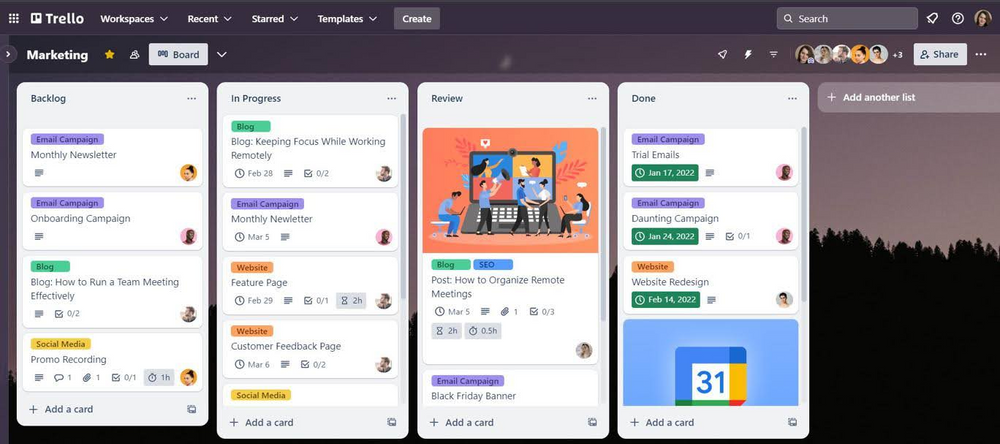
\includegraphics[width=0.8\textwidth]{imagens/trello.png}
    \caption{Interface da plataforma Trello}
    \label{fig:trello}
    \fonte{Elaborado pelos autores (2026).}
\end{figure}

\subsection{Notion}

O Notion é uma plataforma de documentos e bancos de dados muito flexível. Ele tem plano gratuito, e o plano \textit{Plus} custa US\$ 10,00 por membro ao mês na cobrança anual \cite{notion2026}. Como não tem estrutura própria para cursos, o usuário precisa criar e manter os seus próprios bancos de dados, o que toma tempo de configuração.

\begin{figure}[H]
    \centering
    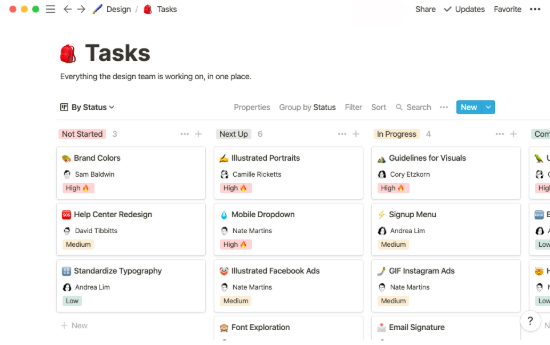
\includegraphics[width=0.85\textwidth]{imagens/notion.png}
    \caption{Interface da plataforma Notion}
    \label{fig:notion}
    \fonte{Elaborado pelos autores (2026).}
\end{figure}

\subsection{Asana}

O Asana é voltado à gestão de projetos por tarefas. O plano \textit{Starter} custa US\$ 10,99 por usuário ao mês na cobrança anual \cite{asana2026}. Ele traz recursos pensados para equipes, como o controle da carga de trabalho de cada pessoa, que servem pouco ao criador individual, e não foi feito para o fluxo de produção de cursos.

\begin{figure}[H]
    \centering
    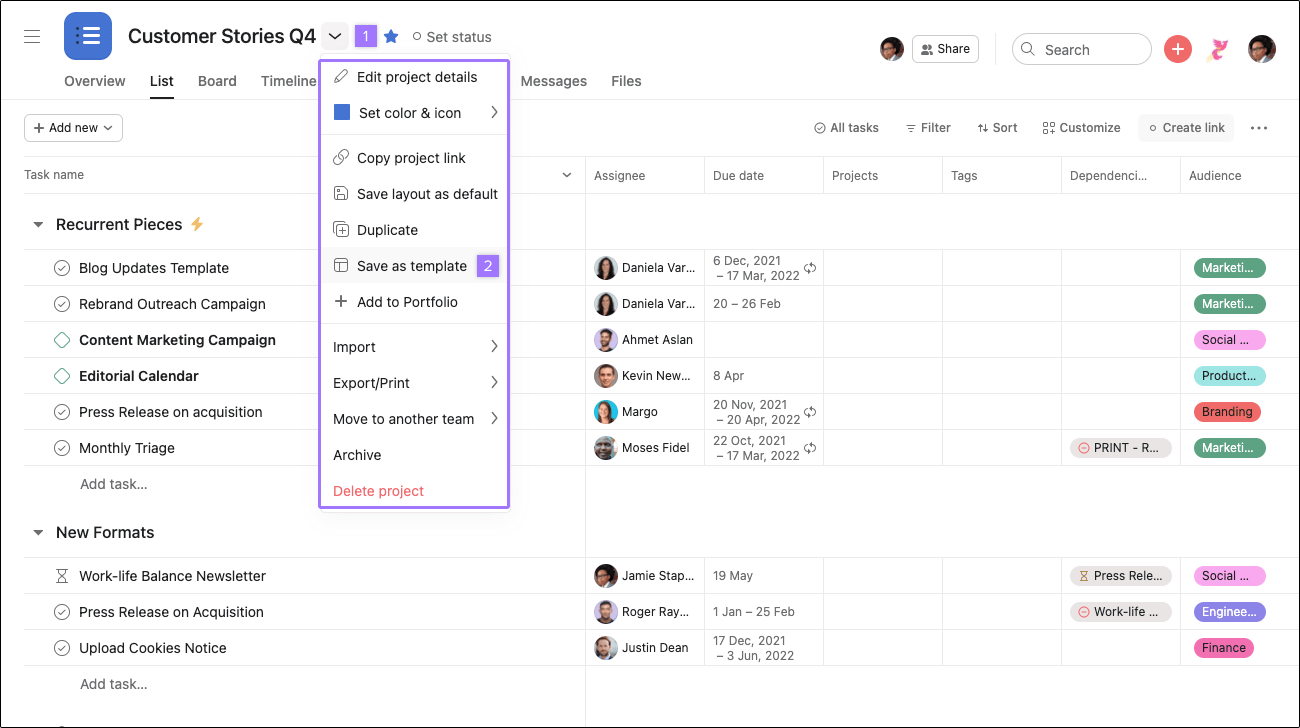
\includegraphics[width=0.85\textwidth]{imagens/asana.png}
    \caption{Interface da plataforma Asana}
    \label{fig:asana}
    \fonte{Elaborado pelos autores (2026).}
\end{figure}

\subsection{Comparativo}

A Tabela~\ref{tab:comparativo} compara as plataformas. Os preços em reais foram convertidos pela cotação PTAX de venda de 28/10/2026 (R\$ 5,3420) \cite{bcb2026}. O preço do Creator Workbench é o do plano pago mais barato (Solo), com cobrança mensal. Os preços dos concorrentes são os da cobrança anual.

\begin{table}[H]
\centering
\small
\caption{Comparativo entre plataformas (consulta em 03/11/2026)}
\begin{tabular}{|p{3.6cm}|p{2.2cm}|p{2.2cm}|p{2.2cm}|p{2.6cm}|}
\hline
\textbf{Recurso} & \textbf{Trello} & \textbf{Notion} & \textbf{Asana} & \textbf{Creator Workbench} \\
\hline
Foco Educacional & Baixo & Médio & Baixo & Alto \\
\hline
Estrutura de Cursos & Não & Manual & Não & Nativo \\
\hline
Gestão de Materiais & Link externo & Interno & Link externo & Integrado \\
\hline
Custo (plano pago básico, por usuário/mês) & US\$ 5,00 (R\$ 26,71) & US\$ 10,00 (R\$ 53,42) & US\$ 10,99 (R\$ 58,71) & R\$ 49,00 (plano Solo) \\
\hline
Plano gratuito & Sim & Sim & Sim & Sim (plano Gratuito limitado e teste grátis de 14 dias dos planos pagos) \\
\hline
Interface em português (Brasil) & Sim & Sim & Sim & Sim \\
\hline
Campos próprios para roteiro & Não & Manual & Não & Nativos \\
\hline
\end{tabular}
\label{tab:comparativo}
\fonte{Elaborado pelos autores com base em \cite{trello2026,notion2026,asana2026,bcb2026}.}
\end{table}